\chapter{Cloud macrophysical and radiative properties observed during the Norwegian Young Sea Ice field campaign}
\vspace{1 cm}
\begin{spacing}{1} \begin{quote} 
\noindent \emph{The combined effect of all climate feedback processes is to amplify the climate response to forcing (virtually certain). While major advances in the understanding of cloud processes have increased the level of confidence and decreased the uncertainty range for the cloud feedback by about 50$\%$ compared to AR5, clouds remain the largest contribution to overall uncertainty in climate feedbacks (high confidence).} \end{quote}
\hspace{6 cm} - IPCC Sixth Assessment Report, August 2021  
\end{spacing}
\doublespacing
\section{Introduction}
The global climate is heavily influenced by processes that occur in the Arctic. However, the Arctic environment is currently experiencing rapid change \citep{overland:2011, stroeve:2007}. Due to a lack of observations, it has been difficult to fully understand atmospheric processes in the polar regions \citep{persson:2002}. The atmospheric circulation in the Arctic is modified by changes in the overall climate, which, in turn, impact cloudiness and radiation at the surface \citep{zhang:2008}. The Advanced Very High-Resolution Radiometer (AVHRR) has observed that wintertime cloud cover over the Arctic Ocean is decreasing by 5$\%$ per decade. Meanwhile, in spring, increases as large as 15$\%$ per decade have been observed, which can likely be attributed to changes in atmospheric circulation \citep{schweiger:2004}. A decreasing trend in Arctic sea ice of 2.9$\%$ to 9.1$\%$ per decade was seen from 1979 through 2006 \citep{stroeve:2007}. Measurements of the energy balance and cloud properties (fraction, height, microphysical, and temperature) can give important insight into climate processes and radiative transfer but are rarely measured together \citep{persson:2002, schweiger:2004, miller:2017}. 

Clouds change the surface temperature by modifying both the shortwave and longwave radiation reaching the surface. Cloud microphysics, such as phase and particle size, as well as macrophysics, including fractional coverage, cloud height, and thickness, can influence the amount of radiation reaching the surface and, in turn, influence the impact of the cloud-radiation feedback \citep{uttal:2002}. This relationship is nonlinear and depends on both cloud and sea ice characteristics \citep{intrieri:2002}.

Clouds, as stated above, can modify both the radiation budget and impact the ice-albedo feedback. The influence of clouds is magnified by the high surface albedo and the lack of atmospheric moisture \citep{shupe:2003}. While we do have some estimates on how much the clouds can impact these feedbacks, more information is needed to quantify the exact influence. \citet{sledd:2019} states that the clouds are the most important driver in changes in top-of-atmosphere albedo over the entire globe, including at the poles, regardless of the high surface albedo. Cloud characteristics were shown to directly impact the ice thickness in studies by \citet{curry:1992, beesley:2007}.  

The impact of clouds is often quantified using cloud radiative forcing (CRF). The CRF describes how clouds modify the radiation at the surface by taking the difference between the observed all-sky radiation and the estimated clear-sky radiation \citep{ramanathan:1989}. When positive radiative forcing is observed, there is a surplus of net radiation at the surface under cloudy skies, and they drive warming. When the CRF is negative, cooling occurs at the surface under clouds. During clear skies, CRF should equal zero, as the actual radiation should be the same as the estimation of clear-sky radiation. Clear-sky radiation is often calculated from a radiative transfer model or estimated using observed clear-sky times.

Net cloud radiative forcing is a balance of surface warming and cooling due to modifications in radiation as a result of cloud cover. \citet{curry:1992, intrieri:2002} found that in the Arctic, clouds warm the surface over the entire year (have a positive cloud radiative forcing) except for in mid-July, when the sun is high above the horizon and the surface albedo is relatively low. This nearly year-round warming is due to the small amount of shortwave radiation. When there is solar radiation present, the low sun elevation angle and high surface albedo reflect much of the shortwave radiation away. In addition, the low-level clouds are often emitting longwave radiation at warmer temperatures than the ice surface due to surface temperature inversions \citep{shupe:2003} and are always emitting more effectively than the clear sky.

The Norwegian Young Sea Ice Experiment (N-ICE2015, or N-ICE) \citep{granskog:2018} is the first experiment to make comprehensive measurements of clouds and the surface energy balance from winter to summer since the Surface Heat Budget of the Arctic Ocean Experiment (SHEBA) in 1997 and 1998 \citep{walden:2017, uttal:2002}. While N-ICE was conducted north of Svalbard in the Arctic Ocean, SHEBA took place north of Alaska in the Beaufort and Chukchi Seas, measuring the components surface energy budget \citep{persson:2002, andreas:2010, grachev:2007}, cloud properties \citep{turner:2005, turner:2002, intrieri:2002, shupe:2004}, and the resulting surface properties \citep{intrieri:2002, shupe:2004}. 

SHEBA was conducted almost two decades before N-ICE. Measurements were taken further into the ice pack \citep{cohen:2017} and in thicker ice conditions. In addition, the meteorological conditions were different; detailed comparisons of N-ICE and SHEBA during the winter can be found in \citep{graham:2017:comp}. There were a few warm events during N-ICE caused by synoptic storms when temperatures reach 0 $^{\circ}C$; these events were much warmer than any of the warm periods experienced during SHEBA.  During the warm periods at N-ICE, the cloud properties were quite variable, suggesting that some of the changes in the surface energy balance could be the result of changes in cloud macrophysical and/or microphysical properties. Throughout SHEBA, mixed-phase clouds were observed 41$\%$ of the time. \citet{graham:2017:comp} states that in the winter, extreme radiative cooling events were more frequent during the N-ICE period than during SHEBA. More information about N-ICE can be found in Chapter 2.

Due to their importance to the surface energy budget over the Arctic Ocean, it is important to investigate the properties and radiative forcing of clouds during N-ICE and to compare the results to those observed during SHEBA. These results will provide useful constraints for models that traditionally have had difficulty simulating radiation at the surface of Arctic sea ice. Proper modeling of Arctic clouds in all seasons is essential for simulating accurate values of the surface energy budget, which is critical for modeling the seasonal cycle of sea ice. A critical parameter that was identified during SHEBA \citep{inoue:2008, tjernstrom:2005} and other Arctic field experiments \citep{hines:2017, listowski:2017, hines:2019} is the fraction of mixed-phase clouds. \citet{graham:2019} showed that six atmospheric reanalyses have difficulty simulating Arctic clouds.

This paper uses various observations obtained during the N-ICE2015 field campaign to document the cloud macrophysical properties, the shortwave (SW) and longwave (LW) radiation, and the net cloud radiative forcing (CRF) at the surface of young Arctic sea ice. Section 2 describes the various measurements that were made during N-ICE to estimate CRF. Section 3 describes the methods to calculate CRF, which involved combining N-ICE measurements with radiative transfer modeling. Section 4 describes the seasonal transition of CRF from winter to summer. Section 5 compares the calculated CRF to modeled CRF in two model simulations. Section 6 presents the conclusions of this study.

\section{Measurements}
N-ICE was conducted during the six-month transition from winter to summer (January - June 2015) in the Arctic Ocean north of Svalbard. All of the instruments were either deployed onboard the Norwegian research vessel Lance or on the sea ice near the Lance. The instruments used in this study were a Vaisala CL-25 ceilometer, a Micropulse Lidar (MPL), twice-daily Vaisala RS92-SGP radiosondes, and Kipp and Zonen shortwave and longwave broadband radiometers. More information about N-ICE can be found in Chapter 2. 

The synoptic context of the N-ICE field campaign is described by \citet{cohen:2017}. The storms designated in Table 2 of \citet{cohen:2017} are of particular interest to this study. Six major and three minor storms occurred in winter (between 21 January and 14 March), while two major and seven minor storms occur in spring and summer (from 23 April through 11 June). The winter was characterized by a succession of particularly strong storms (as compared to climatology), while the spring conditions were typical of that region of the Arctic \citep{graham:2017}. The winter storms were accompanied by large increases in the integrated water vapor and changes in wind direction \citep{kayser:2017} that influenced cloud properties.

A list of the meteorological instrumentation deployed during N-ICE is given in Table 1 of \citet{cohen:2017}. A thorough description of the Vaisala RS92-SGP radiosondes launched during N-ICE is given by \citet{kayser:2017}. A brief description of the meteorological measurements is given here as they pertain to this study.

Radiosondes were launched from the ice surface (Floe 1) and from the ship deck (Floes 2, 3, 4) to measure vertical profiles of temperature, relative humidity, wind speed and direction, pressure, and geopotential height up to a maximum altitude of 30 $km$. More information and analysis of the radiosondes can be found in \citep{kayser:2017}. Here the radiosonde profiles were combined with the surface and tower meteorological measurements to create input files for a radiative transfer model (section 3.2).

A MPL was used to measure backscattered radiation and depolarization from aerosols and clouds along the vertical path of the lidar beam \citep{spinhirne} throughout the N-ICE field campaign. The MPL was mounted on the upper deck of the R/V Lance and was approximately 10-12 meters above the sea ice surface. The MPL \citep{campbell:2002} is a Sigma Space Version 4 polarization-sensitive lidar (532 $nm$) that was provided by the U.S. Department of Energy’s (DOE) Atmospheric Radiation Measurement (ARM) Program. Raw MPL data was collected at 5-second temporal resolution and 15-meter spatial resolution up to an altitude of 18 km above the surface. The uncertainty in the base height of clouds (derived from MPL measurements) is $\pm$ 2 $\%$ due to timing uncertainties within the instrument. The lidar beam is attenuated more by water droplets than ice particles, so our determination of the cloud fractions of water and ice clouds is biased toward a higher percentage of water than ice. In addition, the MPL signal is highly attenuated by optically thick clouds, so when a low thick water cloud is detected, it is possible that additional cloud layers may exist above this layer that is not detected by the MPL. In these cases (which occur often in spring and summer), we assume that the low thick cloud layer is solely responsible for the cloud radiative forcing at the surface. Post-processing of the MPL measurements is described below in section 4.3.1 and is based on the analysis methods of \citet{campbell:2002}, \citet{flynn:2007}, and \citet{stillwell:2018}.

Broadband radiometers were deployed at 1 to 1.2 $m$ above the surface near the meteorological tower to measure upward and downward components of longwave (Kipp and Zonen CGR4) and shortwave (Kipp and Zonen CMP22) radiation. Kipp and Zonen CVF4 ventilation units were used to heat and ventilate the radiometers to avoid frosting of the instrument domes during periods of high relative humidity. The surface skin temperature was calculated from the upwelling and downwelling longwave radiation, assuming a broadband surface emissivity of 0.99 \citep{grenfell:1999}; the surface skin temperature was used as input for radiative transfer modeling. More information about the radiometers, including analysis of the surface energy budget, can be found in \citet{walden:2017}.

In spite of deploying a relatively comprehensive instrument suite over sea ice during N-ICE2015, there are some caveats regarding these measurements. Most importantly, when the optical depth of the overlying clouds is large, the MPL is unable to penetrate completely through the clouds. This is especially true when liquid water clouds are present, which occur often in spring and summer and occasionally in winter. Thus, the cloud macrophysical properties that are reported here represent only the lowest layer of cloud cover in many cases. It would have been preferable to also deploy a cloud radar, which is less sensitive to liquid water, that would have profiled clouds above any liquid layers. Other additional instruments would have been useful for measuring the liquid water path (microwave radiometer) and cloud microphysical properties (infrared spectrometer, cloud radar). So given the instruments that were deployed, we report on both the cloud macrophysical properties (within the capability of the MPL) and cloud radiation, with a focus on surface cloud radiative forcing, which is most sensitive to the lowest cloud layer. 

\section{Methods}
In this study, the macrophysical and radiative properties of clouds are described throughout the N-ICE2015 field campaign. Below we explain how cloud base height, temperature, fraction, and cloud radiative forcing are derived from the instruments deployed during the field campaign.

\subsection{Cloud Macrophysical Properties}
Measurements from the MPL and routine radiosonde launches during N-ICE provide estimates of three macrophysical cloud properties: cloud fraction, temperature, and phase. Raw data from the MPL were corrected for pulse pileup (saturation) and background light (from sky and/or detector dark noise), creating “background-subtracted raw counts”. Several additional corrections are then applied: afterpulse calibration, daily normalization to the median laser pulse energy, and an overlap correction to remove the effect of range-dependent collection efficiency of the fiber-coupled receiver  \citep{campbell:2002, micropulse:2006}. Both signal-to-noise (SNR) and speckle filtering was then performed on the data.

Two lidar parameters are then calculated for our analysis: backscatter ratio and polarization. The backscatter ratio is the ratio of total backscattering to molecular backscattering \citep{klett:1981}. The molecular backscattering is estimated using twice-daily radiosonde data. The radiosonde profiles of pressure, temperature, and water vapor were interpolated in time and space to approximate molecular particle number density. Molecular backscattering was then calculated using the Rayleigh scattering approximation \citep{bohren:2006, bohren:2008, placzek:1934}. 

In this study, the backscatter ratio for each lidar volume pixel is used to distinguish clear air from liquid or ice hydrometeors. A volume pixel, or voxel, is a lidar measurement at a particular time and altitude range. Backscatter ratios greater than 7.5 were considered cloudy voxels, while ratios less than 7.5 were identified as clear voxels (including aerosols). The cloud-base height is the lowest altitude a cloud is detected, and the cloud top is the highest. As mentioned above, if the optical depth of the lowest cloud is large, the MPL will only accurately detect the base of the lowest cloud. Once the cloud base is determined, the cloud temperature can be estimated by interpolating the twice-daily radiosonde profiles to the particular time and altitude of the cloud base. The cloud fraction (occurrence) for a given time period is then determined by calculating the fraction of time when a cloud is present vertically overhead.

The polarization of the MPL is calculated using equations 1.4 (depolarization ratio) and 1.5 (depolarization) of \citet{flynn:2007}. These parameters, plus the error in the depolarization ratio, are used to classify the cloudy voxels into three categories: liquid, ice, and unclassified cloud. Cloudy voxels with depolarization ratios greater than 0.1 are classified as ice, while voxels with depolarization ratios lower than 0.1 are liquid. Cloud voxels cannot be classified as mixed-phase and are categorized as liquid versus ice as done in previous lidar studies (e.g., \citet{intrieri:2002}). The classification is further refined using the error in depolarization ratio, requiring this error for liquid and ice to be less than 10 $\%$. If the depolarization-ratio error is greater than 10 $\%$ for the initial classification of liquid or ice, the cloud voxel is classified as an “unclassified cloud”. 

Once each voxel is classified, a column cloud mask is created for comparing the range-resolved lidar measurements with the column measurements made by the broadband radiometers. If the atmospheric column above the lidar lacks clouds at any altitude, the column is considered clear, otherwise, the column is cloudy. Columns containing liquid voxels at any altitude are considered liquid. This implies that a single liquid voxel can override numerous ice voxels. This is done because liquid clouds in the Arctic typically have large optical depths (e.g., \citet{curry:1996}) relative to ice clouds.

\subsection{Cloud Radiative Properties}
The all-sky net radiation at the surface $Q_{all}$ is calculated using 1-hour average radiation measurements from the four Kipp and Zonen radiometers, where the $Q_{all}$ is defined in Eq. \ref{eq:qnet}. $Q_{all}$ is equal to $Q_{net}$ for observations.

\begin{equation}\label{eq:qnet}
Q_{all} = (Q_{lw \downarrow} - Q_{lw \uparrow}) + (Q_{sw \downarrow} - Q_{sw \uparrow})
\end{equation}

$Q_{lw \downarrow}$, $Q_{lw \uparrow}$, $Q_{sw \downarrow}$ and $Q_{sw \uparrow}$ are the components of downward longwave, upward longwave, downward shortwave and upward shortwave radiation. In this paper, positive net radiation is defined as into the surface \citep{miller:2015}.

Cloud radiative forcing is defined in Eq. \ref{eq:crf:1}, \ref{eq:crf:2}, and \ref{eq:crf:3} \citep{ramanathan:1989, miller:2015}.

\begin{equation}\label{eq:crf:1}
CRF = Q_{all} - Q_{clear}
\end{equation}
\begin{dmath}\label{eq:crf:2}
CRF = [(Q_{lw \downarrow} - Q_{lw \uparrow}) + (Q_{sw \downarrow} - Q_{sw \uparrow})]_{all} \\
\\ - [(Q_{lw \downarrow} - Q_{lw \uparrow}) + (Q_{sw \downarrow} - Q_{sw \downarrow})]_{clear}
\end{dmath}
\begin{dmath}\label{eq:crf:3}
CRF = [(Q_{lw \downarrow} - Q_{lw \uparrow})_{all} - (Q_{lw \downarrow} - Q_{lw \uparrow})_{clear}] \\
\\ + [(Q_{sw \downarrow} - Q_{sw \uparrow})_{all} -  (Q_{sw \downarrow} - Q_{sw \uparrow})_{clear}]
\end{dmath}

The clear-sky values for both downward longwave and shortwave radiation in Eq. \ref{eq:crf:3} are calculated using the Rapid Radiative Transfer Model (RRTM) \citep{mlawer:1997} because there were too few clear-sky cases during N-ICE2015 to properly estimate the clear-sky flux using the radiation measurements. For SW calculations, it is important to specify the atmospheric concentrations of $N_{2}$ and $O_{2}$ for molecular scattering and $H_{2}O$, $O_{3}$ and $O_{2}$ for molecular absorption. The surface albedo must also be specified as a function of the surface type and solar zenith angle. For LW calculations, the vertical temperature structure must be specified, as well as the concentrations of the primary infrared greenhouse gases ($H_{2}O$, $CO_{2}$, $O_{3}$, $CH_{4}$, $N_{2}O$, $CO$).

 It is important to specify a vertical grid in RRTM that resolves the near-surface temperature structure because near-surface temperature inversions occurred during N-ICE \citep{kayser:2017}. Here we use three layers (surface, 2 $m$, 4 $m$) below 10 $m$, then increasing spacing above 10 $m$: 10 $m$ spacing from 10 to 100 $m$, 100 $m$ from 100 $m$ to 1 $km$, 1 $km$ from 1 to 30 $km$, and 5 $km$ from 30 to 60 $km$. RRTM was run hourly for the entire field campaign.

Here the concentrations of $N_{2}$ and $CO_{2}$ are assumed to be uniformly mixed vertically, while the seasonal variability of the $CO_{2}$ concentration is accounted for by using monthly averaged measurements from Summit Station, Greenland made by the Global Monitoring Division (GMD) from National Oceanic and Atmospheric Administration (NOAA). The profiles of $O_{2}$, $CH_{4}$, $N_{2}O$, and $CO$ are from the sub-Arctic winter standard atmosphere \citep{mcclatchey:1972}. The profiles of $O_{3}$ were measured at Ny-\r{A}lesund, Svalbard, and were interpolated to hourly profiles. The profiles of temperature and humidity were constructed using: 1) the sensors at 2 $m$ and 4 $m$ on the meteorological tower, 2) the radiosondes from 10 $m$ to the altitude of the balloon burst, and 3) values from the sub-Arctic winter standard atmosphere from the maximum altitude of the radiosonde to 60 $km$. On a few occasions, the termination height of the radiosonde was low (below 10 $km$). In these cases, the monthly average sonde profiles were used from the maximum altitude of the sonde through 24 to 30 $km$ depending on the month. The surface skin temperature was derived from the longwave radiation \citep{walden:2017} and assumed a surface snow emissivity of 0.99 \citep{persson:2002, grenfell:1999}.

The meteorological tower data were compared to the lowest 10 $m$ measured by the radiosondes as a quality check because of the strong dependence of longwave CRF on the near-surface temperature structure. The difference between the 2$-m$ temperature measured on the meteorological tower and the temperature interpolated between radiosondes exceeded 1$^{\circ}C$ in only 1.2$\%$ of the hourly profiles. The other levels (2, 4, and 10 $m$) exceeded a 1$^{\circ}C$ difference of less than 0.5$\%$ of the time. To ensure the lower profiles were as accurate as possible, the tower temperatures and surface temperatures calculated from LW fluxes were used when available but did not change the lower levels of the profiles significantly. Linear interpolation between the tower and sonde measurements was sufficient to represent the lower atmosphere because the altitude range of these temperature adjustments was small ($<$10 $m$).

\begin{figure}[b!]
    \centering
    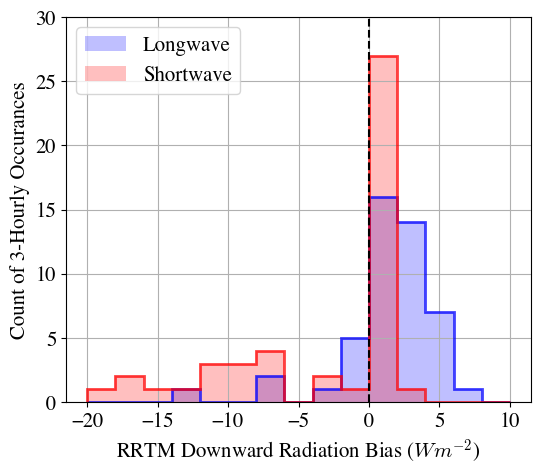
\includegraphics[width=0.65\linewidth]{figures/chapter4/RRTMcorrelation_bias.png}
    \caption[RRTM modeled downward flux bias histogram.]{RRTM modeled downward longwave flux bias (RRTM - observations) in blue and downward shortwave flux bias in red. Three-hourly values during clear-sky times only are shown.}
    \label{fig:rrtm}
\end{figure}

The shortwave spectral surface albedo was estimated using the snow albedo model described by \citet{wiscombe:1980}; see their Eq. 4. This model depends on properties of the snow (single-scattering albedo ($\omega$) and asymmetry factor ($g$)), as well as the solar zenith angle ($\theta$). The single-scattering albedo was determined for each day using noontime albedo measurements from \citet{walden:2017}. A fixed value of $g$ = 0.9 was used. These values were then used along with the hourly solar zenith angle to calculate the albedo throughout the day. The cloud cover also greatly affects the surface albedo, and the reduction in direct radiation in favor of diffuse was parameterized using a diffuse fraction. \citet{key:2001} states that the albedo of ice is 4 to 6$\%$ higher under cloudy skies than clear skies with a range of 0 to 15$\%$. Cloud fraction for the two-hour period surrounding the time of the albedo calculation was used to determine the percent reduction required to account for the diffuse fraction. Percent reductions in albedo were scaled linearly from 6 to 0$\%$, with full cloud cover having a 6$\%$ reduction imposed, and clear sky remaining unchanged.

Uncertainties are introduced into RRTM shortwave and longwave calculations from uncertainties in the albedo estimates, atmospheric profile construction and interpolation, and the various measurements. Despite this, the RRTM calculations agree well with the few clear-sky SW and LW measurements from N-ICE2015. Figure \ref{fig:rrtm} shows a histogram of the differences in SW and LW radiation (modeled minus measured) for clear days. The mean SW bias is -2.5 $W m^{-2}$ with a standard deviation of 9.6 $W m^{-2}$, while the mean LW bias is 1.3 $W m^{-2}$ with a standard deviation of 3.6 $W m^{-2}$. Thirteen three-hour periods that appeared clear in the data were removed as they were at the start of an observation period (the beginning of a floe). These periods had significant differences but, because these were some of the first measurements during their respective floes, they were removed due to the potential for instrument error.

\section{Results and Discussion}
The conditions observed at N-ICE were unique not only because it observed the transition season for the first time since SHEBA. Winter storm periods were measured that brought extremely large and rapid transitions of cloud properties that coincide with changes in turbulent fluxes documented by \citet{walden:2017} and \citet{graham:2017:comp}. 

\begin{figure}[t!]
    \centering
    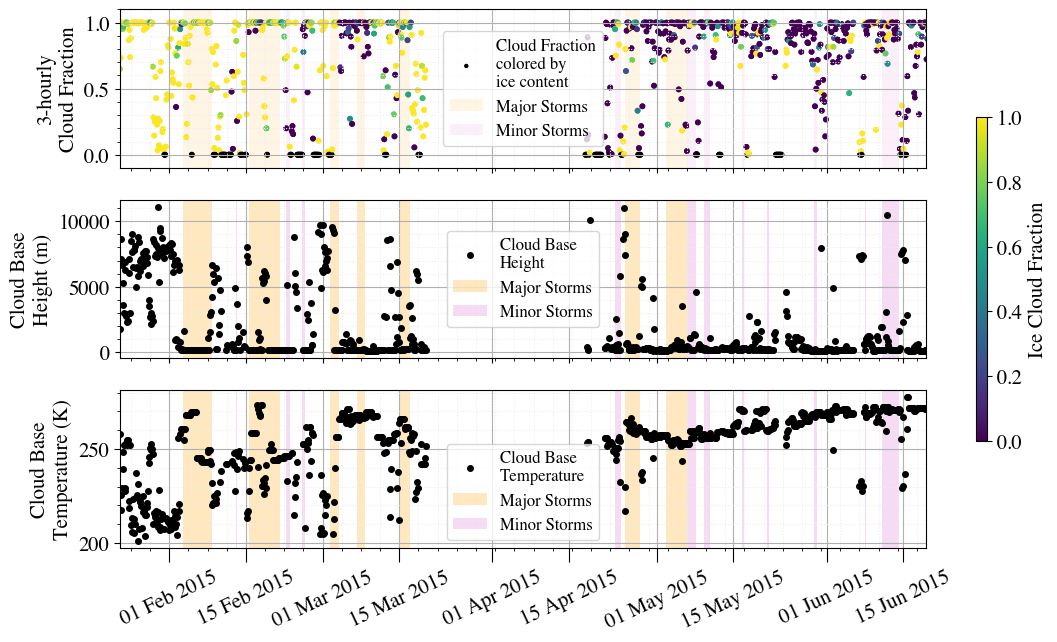
\includegraphics[width=1\linewidth]{figures/chapter4/CloudSummary.png}
    \caption[Cloud fraction and phase, height, and temperature time series.]{Vertical cloud fraction and ice content within the cloud are shown in the top figure. Ice content is defined as the percentage of the cloud that can be determined to be ice particles (yellow represents more ice and purple less). The middle panel shows the 3-hourly mean cloud base height and the bottom panel shows the 3-hourly cloud base temperature. Storm periods are shaded in orange (major) and pink (minor) shading.}
    \label{fig:cloudmacro}
\end{figure}

The upper panel of Figure \ref{fig:cloudmacro} shows the frequency of cloud occurrence, or the percentage of the day that cloud was observed over the MPL, indicated by colorful dots. The color indicates the ice cloud fraction or the percentage of the observed clouds that could be definitively categorized as ice. During the first half of the experiment in winter, it was common for days to have cloud fractions below 50$\%$, with 16 out of the 61 days prior to the long break in observations having less than 50$\%$ cloud cover. After the break, however, there are only 12 days out of the 89 days that are below 50$\%$ cloud cover. The mean cloud fraction during the first half of the experiment is 70$\%$ (standard deviation of 30$\%$), and after is 75$\%$ (standard deviation of 28$\%$). Climatologically, a decrease in clear days has been seen for this region, contributing to a long-term warming trend \citep{kayser:2017}. The entire experiment, including a large number of cloudy days, is put into climatological context by \citet{graham:2017} and \citet{kayser:2017}. For the purpose of this study, there was significantly less cloud cover in winter than in the spring and summer, and the clouds observed during winter had larger ice content than those observed during spring.

During Floes 1 and 2 (winter), every day has at least some ice cloud present. Most of the days have primarily ice clouds with the exception of a week in early March, which corresponds to a period when the cloud base was low (Figure \ref{fig:cloudmacro}, middle panel) and cloud temperature was near freezing (265 - 270 $K$, Figure \ref{fig:cloudmacro}, bottom panel). Some days have a small percentage of unknown cloud fraction, but this category only exceeds 20$\%$ of the daily cloud existence once during the first half of the experiment. 

\begin{figure}[b!]
    \centering
    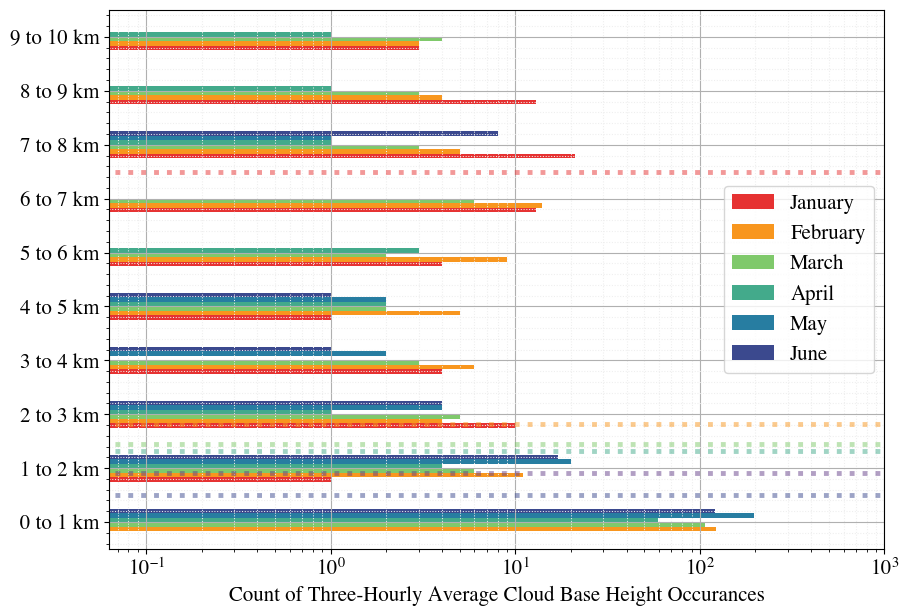
\includegraphics[width=1\linewidth]{figures/chapter4/CloudHeights.png}
    \caption[Cloud base height by month histogram.]{Binned cloud base height by month. Frequency distributions are shown as bars colored by month. The monthly mean cloud height is shown by the horizontal line in the corresponding color. Note the x-axis is shown as a log scale to make differences more clear.}
    \label{fig:cloudbase}
\end{figure}

The fraction of water clouds greatly increases during Floes 3 and 4 (spring and summer). These results are not surprising, as increasing temperature and increasing water fraction are expected. There are still ice clouds present nearly every day through the end of the experiment, many of which are high, thin clouds. The water clouds, however, were primarily thick and close to the surface. Some of the ice can be attributed to mixed-phase clouds with both water and ice through the mid-troposphere. Low-level ice clouds were not common during this period.

Cloud base heights (Figure \ref{fig:cloudmacro}, middle panel) in the first month of the experiment are, on average, higher than the rest of the experiment. Once Floe 3 starts cloud base heights are almost always below 2 $km$. Figure \ref{fig:cloudbase} shows the frequency of cloud base heights for each month throughout the experiment with lines indicating the mean cloud base height. The mean height for January, which includes only a 10-day, relatively quiescent period, is 6.45 $km$, while the rest of the months' mean cloud heights are below 2 $km$. Mean cloud heights decrease throughout the experiment, with the lowest mean cloud base height present in May at just below 1 $km$. During the second half of the experiment, the majority of the clouds have a low cloud base height and a high percentage of water present. These clouds had large enough optical depths that they caused complete attenuation of the micropulse lidar beam, resulting in an inability to view clouds above them. As mentioned above, this inhibits the ability to report on higher-level clouds but does not impact the ability to understand the surface energy budget, as these low-level clouds are the most radiatively important.

Cloud base temperature closely mimics the cloud base height for the majority of the experiment. During the second two floes, the cloud base temperature gradually approaches freezing while the cloud base height stays fairly consistently near the surface. This slow increase in cloud base temperature reflects the increase in atmospheric temperature as more solar radiation reaches the Arctic. 

\subsection{Cloud Radiative Properties}
This section describes the variations in shortwave and longwave fluxes measured throughout N-ICE2015. These fluxes are used to calculate the shortwave, longwave, and net CRF throughout the campaign as defined by Eq. \ref{eq:crf} above. These measurements are then categorized according to the cloud macrophysical properties described above.

\begin{figure}[h]
    \centering
    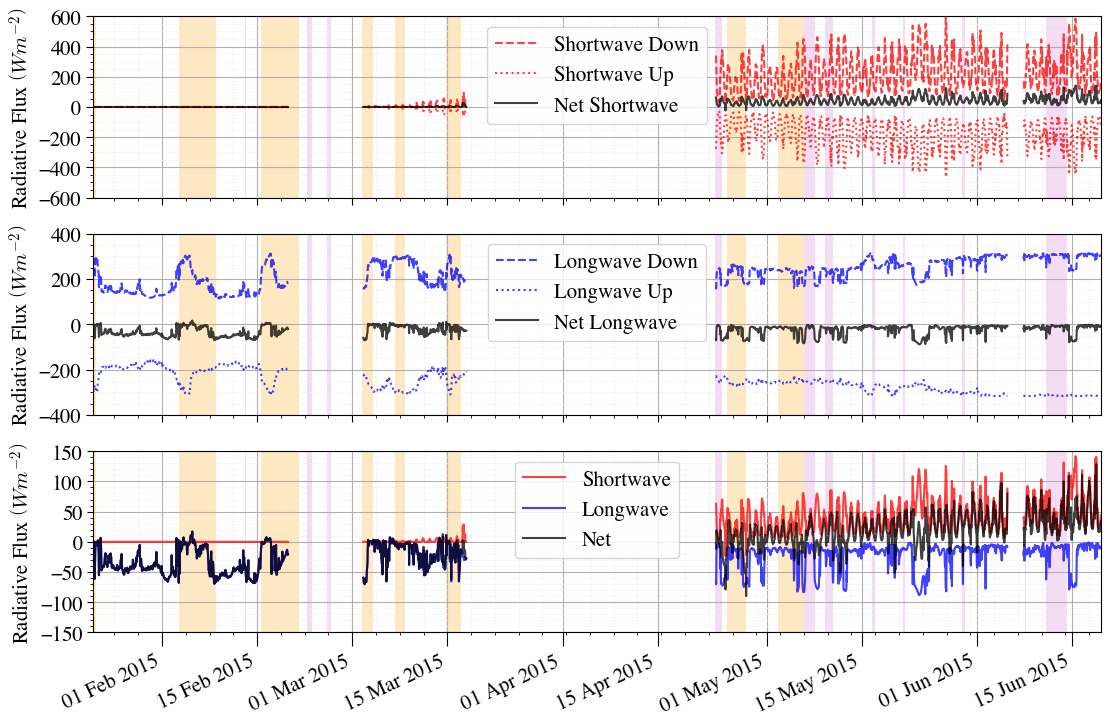
\includegraphics[width=1\linewidth]{figures/chapter4/RadComp.png}
    \caption[Shortwave, longwave, and net radiative components of flux.]{Shortwave (top), longwave (middle), and net (bottom) components of radiative flux. Black lines represent net flux, dotted indicating upward flux, and dashed downward. Major and minor storm periods are shown by the orange and pink shading, respectively.}
    \label{fig:flux:all}
\end{figure}

Figure \ref{fig:flux:all} shows the time series of the shortwave (upper panel), longwave (middle panel), and net (lower panel) radiative fluxes. During Floe 1 (January and February), net flux (also, net longwave flux) dips to around -50 $Wm^{-2}$ during non-storm periods (unshaded) and approaches 0 $Wm^{-2}$ during storm periods (shaded). During major winter storms, downward longwave flux increases from between 100 and 150 $W m^{-2}$ to around 300 $Wm^{-2}$, sometimes within only a few hours. Upward longwave flux mirrors these changes decreasing from -200 to -300 $Wm^{-2}$. During non-storm periods, the upward flux is around -200 $Wm^{-2}$ while the downward flux is just over +100 $Wm^{-2}$, resulting in negative net flux. When the net flux approaches zero, as it does during storm periods, it indicates that clouds are relatively low and warm and have a large enough optical thickness to balance the longwave flux coming from the surface.

In March (Floe 2), the downward and upward longwave fluxes more closely balance each other. This is due to a generally higher downward longwave flux from warmer cloud base temperatures and higher optical thicknesses from a greater fraction of liquid water clouds (Figure \ref{fig:cloudbase}, top panel). During non-storm periods, the net longwave flux reaches a minimum just below -50 $Wm^{-2}$ but is more frequently around -25 $Wm^{-2}$. Storm periods continue to bring the net flux near 0 $Wm^{-2}$, as lower and warmer clouds predominate. Small amounts of shortwave flux exist during the end of this floe (net $< 50~Wm^{-2}$) as the sunlight returns to these latitudes, but has little influence on net flux due to a large amount of reflected shortwave flux from the surrounding snow.

During Floe 3 (spring), the net longwave flux reaches as low as -70 $Wm^{-2}$ but is more often around 0 $Wm^{-2}$. This is the result of increased and consistently high downward longwave flux. This is when the atmosphere is in an opaquely cloudy state \citep{stramler:2011, graham:2017}. As the experiment transitioned from winter into spring, cloud base height decreased and cloud occurrence increased. The decrease in cloud height and warming of the atmosphere results in an increased downward longwave flux from the clouds. In addition, during this period, the floe drifted into warmer ocean water \citep{kayser:2017} and the net shortwave flux increased, which increased the atmospheric temperature above the ice and the magnitude of the upward longwave flux. Upward longwave radiation is fairly consistent throughout this floe, starting around -225 to -250 $Wm^{-2}$ in late April and steadily increasing in magnitude to around -300 $Wm^{-2}$ in June. During this period, the upward longwave flux does not mirror the downward longwave flux as closely as it does during winter, especially as the surface temperature approaches freezing ($Q_{LW\uparrow} \approx 316~W~m^{-2}$).

The net shortwave flux during Floe 3 generally fluctuates between 0 and 100 $Wm^{-2}$, with only 6 days exceeding 100 $Wm^{-2}$. The total net flux follows the daily pattern of the net shortwave flux and is primarily greater than 0 $Wm^{-2}$. During the start of this floe, net flux drops below 0 $Wm^{-2}$ during the two major storm periods. These drops are caused by both a decrease in net shortwave flux (due to increased cloud optical thickness) and a decrease in net longwave flux (higher cloud base and lower cloud base temperature, Figure \ref{fig:cloudmacro}). After this, there are a few more occurrences in which the flux decreases below 0 $Wm^{-2}$, which coincide with decreases in the net longwave radiation, indicating higher cloud bases and/or lower cloud fractions (Figure \ref{fig:cloudmacro}). It is important to note that the clear-sky modeled radiation was estimated to be slightly less than the measured radiation, resulting in clear-sky periods being slightly negative in some cases. This can be seen in the first floe when the upward longwave CRF is slightly below zero, creating a negative CRF. This does not mean that clouds were cooling the surface at this time but is a result of the modeled clear-sky uncertainty. 

June (Floe 4) experienced the greatest magnitude of net flux. Only two days (23 May and 15 June) had a daily average flux larger than 350 $Wm^{-2}$. These days had primarily clear sky conditions. During the storm period from 11 June to 14 June, net longwave flux decreases from 50-75 to about 0 during the storm, and is negative. This occurs at the same time as an increase in cloud base height from near the surface to around 10 $km$ (Figure \ref{fig:cloudmacro}, middle panel). This is the largest decrease in net flux in June. During this time, optically thick clouds block shortwave radiation from reaching the surface. Net longwave flux rose to around 0 $Wm^{-2}$ during this time, keeping net flux above 0 $Wm^{-2}$. After the storm, the net flux increases to about the same magnitude, and the net longwave decreases, becoming more negative after the storm passage than before. This corresponds to an increase in cloud base height, a decrease in cloud base temperature, and a decrease in the cloud fraction (Figure \ref{fig:cloudmacro}) indicating that, after the storm passed, clouds became high and more scattered, including a day with the lowest cloud fraction in June. 

\begin{figure}[t!]
    \centering
    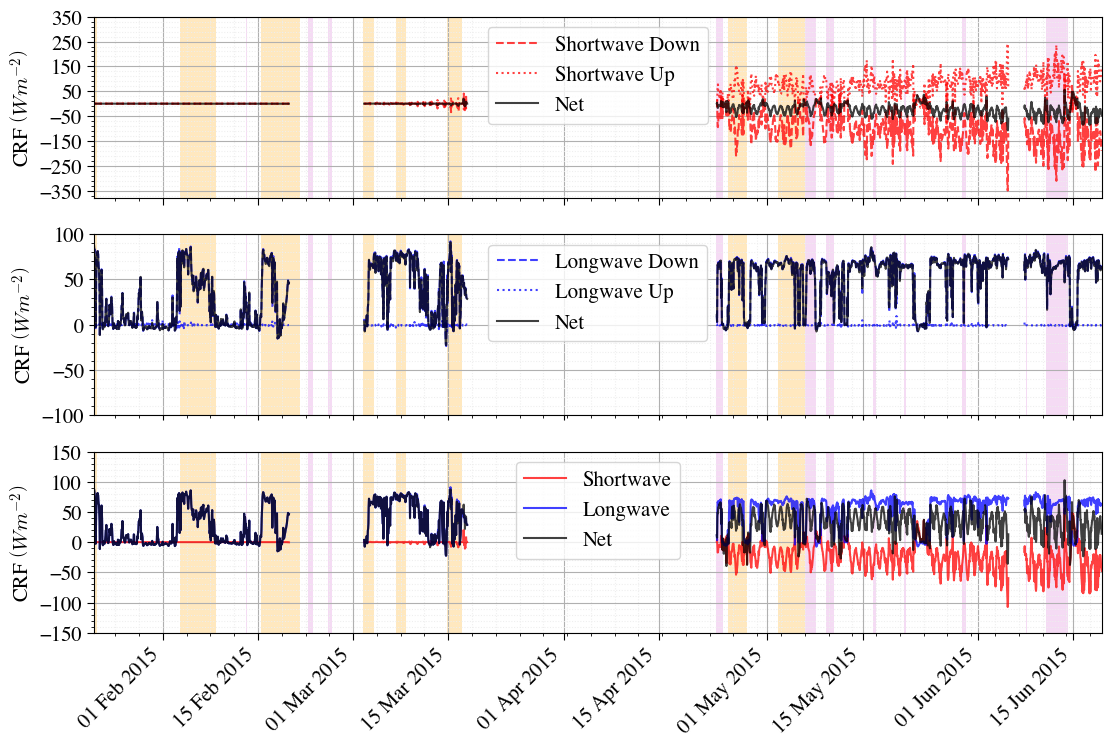
\includegraphics[width=1\linewidth]{figures/chapter4/RadForcing.png}
    \caption[Shortwave, longwave, and net components of cloud radiative forcing.]{Shortwave (top), longwave (middle), and net (bottom) components of cloud radiative forcing. Black lines represent net flux, dotted indicating upward CRF, and dashed downward. Major and minor storm periods are shown by the orange and pink shading, respectively.}
    \label{fig:crf_timeseries}
\end{figure}

Cloud radiative forcing at the surface is shown in Figure \ref{fig:crf_timeseries}. Longwave CRF dominates throughout the field campaign. During Floes 3 and 4, the shortwave CRF has an increasing influence on the net CRF, but only decreases it by a small amount. Upward and downward shortwave CRF counteract each other due to the high albedo of the snow cover on the sea ice, resulting in net shortwave CRF between -50 and 0 $Wm^{-2}$. (\citet{walden:2017} report values of the surface albedo during N-ICE2015.) 

Due to the positive CRF throughout almost the entire field campaign, clouds are generally warming the surface. During SHEBA and other studies \citep{schweiger:2004, cogley:1984, walsh:1998, curry:1996} clouds were found to warm the surface throughout the entire year except in mid-summer when the solar zenith angle was high and albedo low. The length of this cooling period was highly dependent on albedo estimations \citep{intrieri:2002}. As N-ICE did not continue through the entire summer, it is impossible to say if there would be a period of negative cloud radiative forcing later in the summer in this region, when further melt drove the albedo lower. It is true, however, that the net CRF decreased with increasing solar radiation near the end of the campaign.

\begin{figure}[t!]
    \centering
    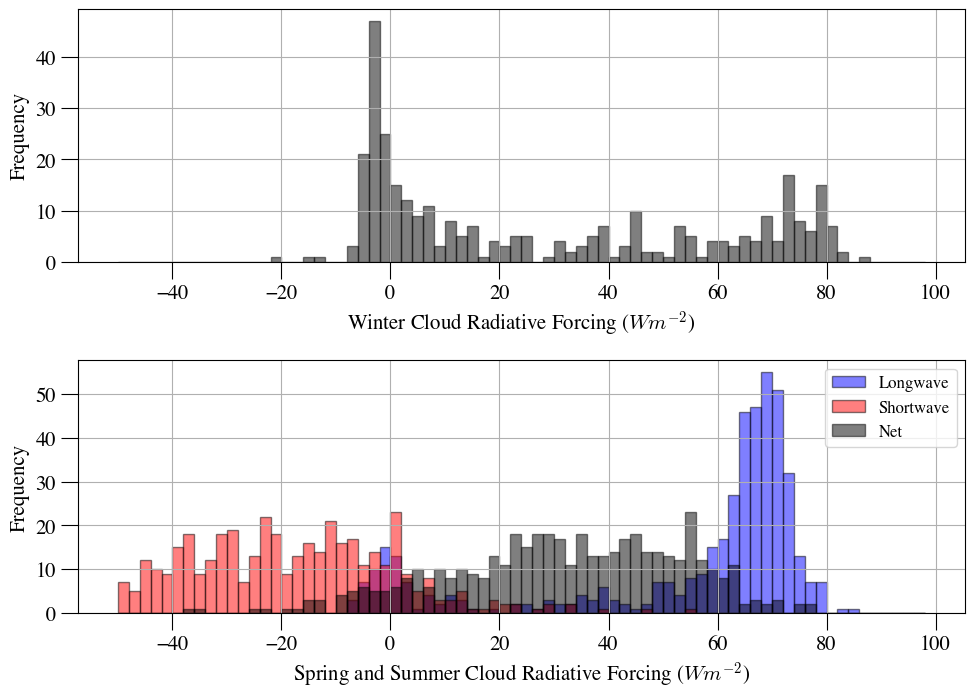
\includegraphics[width=1\linewidth]{figures/chapter4/ForcingValues.png}
    \caption[Histograms of cloud radiative forcing by season.]{Histograms of cloud radiative forcing for winter (top, Floes 1 and 2) and spring/summer (bottom, shortwave radiation indicated in red, longwave in blue, and net in black). Spring/summer is defined as Floes 3 and 4.}
    \label{fig:crf_histo}
\end{figure}

Histograms of the longwave, shortwave, and net CRF, shown in Figure \ref{fig:crf_histo}, are divided by floe. Winter is defined as Floes 1 and 2 and spring/summer is Floes 3 and 4. Shortwave values were very low during the winter floes and are not displayed here. In winter (top panel), the histogram (LW only) shows a slightly bimodal distribution, with one large peak near 0 $W m^{-2}$ and another small peak between about 50 and 80 $W m^{-2}$. (Note that the negative value of the large peak at 3 $W m^{-2}$ may be due to the slight overestimation in the clear-sky flux as the estimated bias is just under 3 $Wm^{-2}$ for shortwave radiation.) These two modes describe clear (0 $W m^{-2}$) and cloudy (75 $W m^{-2}$) conditions. A range of cloud radiative forcing values is seen leading up to the peak of the distribution at about 85 $W m^{-2}$ due to the range in cloud properties (fraction, phase, height) and their associated radiative impacts during the winter. The winter had quite variable cloud conditions compared to those in summer in terms of height, temperature, and daily fraction. The highest winter CRF occurred during the storm periods when cloud fraction was large, clouds were primarily close to the surface and composed of ice, and the cloud base and surface temperatures both increased.  

In the spring/summer (Figure \ref{fig:crf_histo}, bottom panel), the range of net CRF is smaller relative to winter. This is due to the negative shortwave CRF (cooling) that counteracts some of the positive longwave CRF. Longwave CRF in summer is between about 0 $Wm^{-2}$ and 80 $Wm^{-2}$, with the latter (cloudy) peak being the larger of the two (unlike winter). The majority of clouds during summer result in from 50 to 80 $Wm^{-2}$ of longwave CRF. Shortwave CRF ranges between just above zero to -30 $Wm^{-2}$, with a few values as low as -50 $Wm^{-2}$. SW CRF values are the result of the uncertainty in the clear-sky estimations. The result of these two competing components of CRF is a slightly bimodal distribution of net CRF, with a small peak near 0 $Wm^{-2}$ and a larger peak between 30 to 70 $Wm^{-2}$. The peak near 0 $Wm^{-2}$ is small due to the limited number of clear-sky days seen during the summer. Clouds were consistently low and thick throughout the spring and summer, resulting in more uniform net CRF values throughout these two seasons than in winter.

\begin{figure}[p]
    \centering
    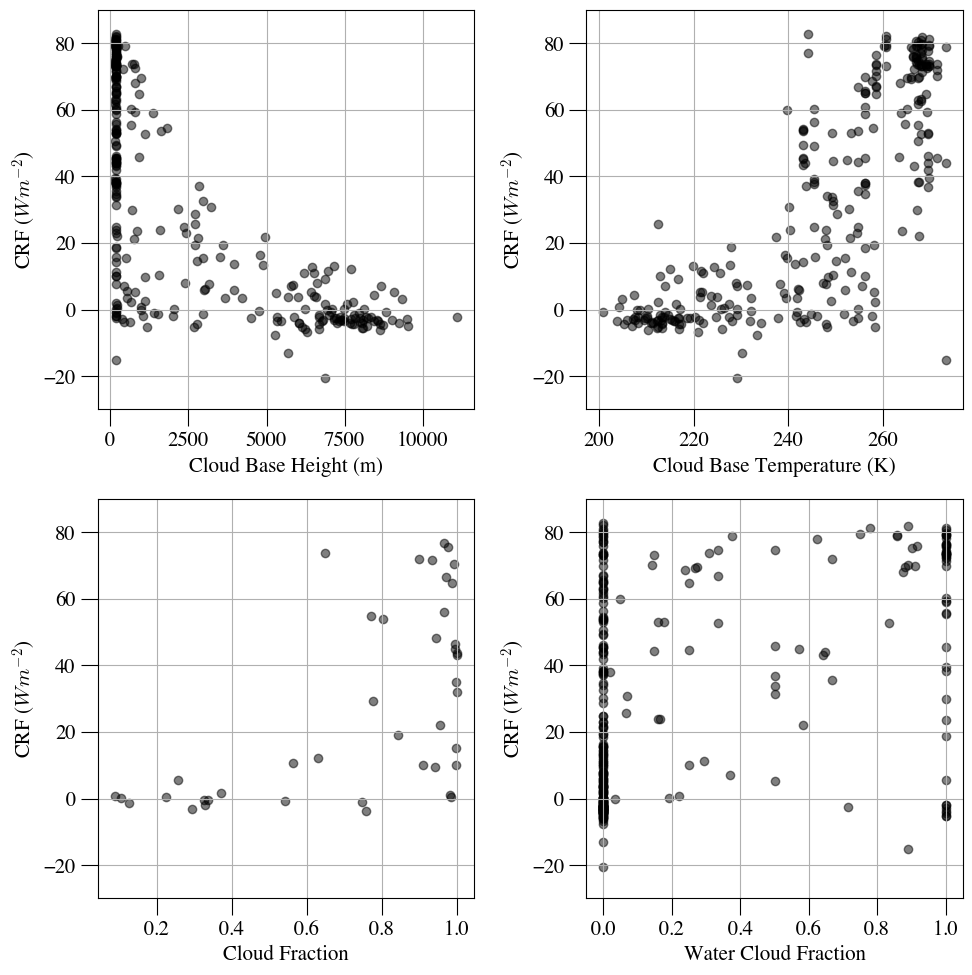
\includegraphics[width=1\linewidth]{figures/chapter4/VSWinter.png}
    \caption[Cloud radiative forcing vs cloud base height, cloud base temperature, cloud fraction, and water cloud fraction for winter.]{Cloud radiative forcing vs cloud base height (top left), cloud base temperature (top right), daily mean cloud fraction (bottom left), and water cloud fraction (bottom right) for the winter season (Floes 1 and 2). All panels are 3-hourly values with the exception of daily mean cloud fraction. Cloud fraction is presented as daily averages to allow for a longer cloud fraction averaging time. Net cloud radiative forcing is only comprised of longwave radiation during this time of year, so black dots represent both the net longwave CRF and the net CRF.}
    \label{fig:winter:crf}
\end{figure}

\begin{figure}[p]
    \centering
    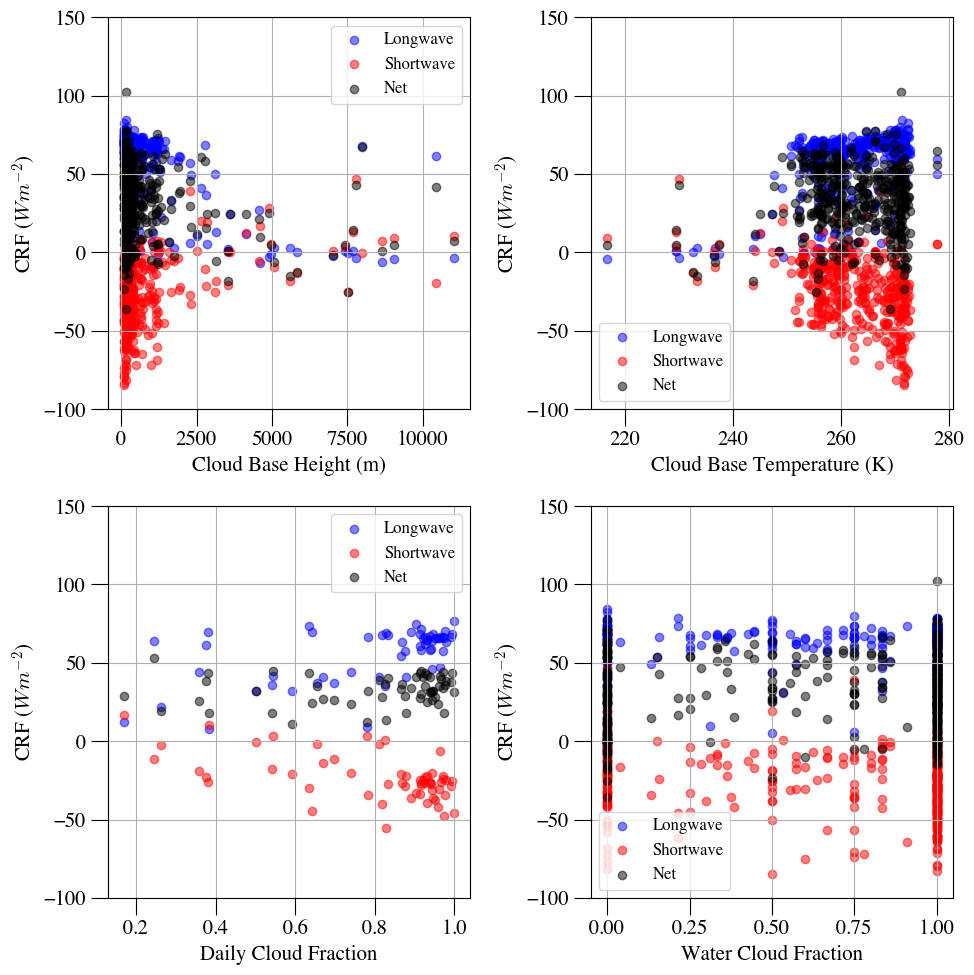
\includegraphics[width=1\linewidth]{figures/chapter4/VSSummer.png}
    \caption[Cloud radiative forcing vs cloud base height, cloud base temperature, cloud fraction, and water cloud fraction for summer.]{Cloud radiative forcing vs cloud base height (top left), cloud base temperature (top right), daily mean cloud fraction (bottom left), and water cloud fraction (bottom right) for the spring/summer season (Floes 3 and 4). Longwave radiation is represented by blue dots, shortwave by red dots, and net by black dots in each scatter plot.}
    \label{fig:spring:crf}
\end{figure}

Figures \ref{fig:winter:crf} and \ref{fig:spring:crf} display how the net cloud radiative forcing depends on the cloud's macrophysical properties. Figure \ref{fig:winter:crf} is for winter (Floes 1 and 2), and Figure \ref{fig:spring:crf} is for spring and summer (Floes 3 and 4). During the winter, cloud base height, and cloud base temperature have the most effect on the net CRF. This is no surprise as the free atmosphere is warmer close to the ground, resulting in low clouds having a larger longwave influence on the surface. \citet{shupe:2004} found that clouds with temperatures cooler than 243 $K$ (-30$^{\circ}C$) often had similar longwave radiative properties to clear sky conditions. In winter at N-ICE, there is a transition in radiative values around 235 $K$. Winter clouds with base temperatures greater than 235 K had a larger spread in cloud radiative forcing values of about 60 $Wm^{-2}$. Values lower than this still had variation in CRF, but were within 20 $Wm^{-2}$ of clear-sky conditions and were more sensitive to changes in cloud base temperature. In the summer, this transition occurred closer to the 243 $K$ cutoff reported by \citet{shupe:2004}. However, due to the limited number of high, cold clouds, there were not many clouds below this threshold. In summer the LW CRF was close to zero for these lower temperatures, in better agreement with the results from \citet{shupe:2004}. 

Daily mean cloud fraction (Figure \ref{fig:winter:crf} and \ref{fig:spring:crf}, lower left panels) does not have as clear of a correlation with daily mean surface CRF.; In the winter, days with below 50$\%$ cloud fraction have less than 10 $Wm^{-2}$ of CRF, while days with cloud fraction greater than 50$\%$ can have CRF values that range from around 0 to just under 80 $Wm^{-2}$. These slight trends were also seen by \citet{shupe:2004} during the SHEBA experiment. 

In spring and summer, the relationships between cloud base height and cloud base temperature are less obvious. This is due to the lack of variety in cloud characteristics during this period and the dependence on solar zenith angle. Most clouds were below 2 $km$ with cloud base temperatures above 250 $K$. Periods of higher, cooler clouds were present only during a few storm periods, one near the end of the experiment. These clouds had a higher ice fraction than the other summer clouds, likely due to their height. 

There is no apparent correlation between the fraction of cloud that is water and the amount of CRF in either season. \citet{schweiger:1999} started that the relationship between particle size and the amount of longwave CRF is not significantly different for liquid and ice particles. They did report a significant difference, however, in shortwave CRF, as the different shapes have different influences on shortwave scattering. However, results from N-ICE do not show differences in water and ice clouds. This is likely due to the inability to determine the thickness of the cloud, as the lidar pulse will attenuate near the base of optically thick clouds, and the wide variety of solar zenith angles that were experienced during the transition to summer. 

The cloud macrophysical and radiative effects seen here could be representative of conditions that are becoming more prominent with climate change. A thorough understanding of the cloud influence on the surface is vital both for forecasting local impacts, such as ice melt or change in surface fluxes, and for use in larger climate circulation models for a more accurate understanding of global climate change. Cloud properties (such as height, phase, and temperature) have a large influence on longwave radiation.

\section{Cloud Radiative Forcing modeled by Polar WRF}
Cloud radiative forcing from the Weather Research and Forecasting model (WRF) with polar enhancements (described in Chapter 3) is shown in Figure \ref{fig:wrf_crf_all}. Two model simulations were selected based on their performance in spring and summer during N-ICE. The model run using the Morrison Bulk Two-Moment cloud microphysics (CM) scheme and the Mellor–Yamada Nakanishi Niino (MYNN) planetary boundary layer (PBL) scheme (2-MYNN, purple) had the lowest biases in latent and sensible heat fluxes in the winter. In the spring, the run with the Goddard CM scheme and Mellor–Yamada–Janjic PBL scheme (G-MYJ, orange) had the lowest biases in latent and sensible heat fluxes and net shortwave flux. For more details about the model setup and the strengths/weaknesses of the PBL and CM schemes, see Chapter 3.

\begin{figure}[t]
    \centering
    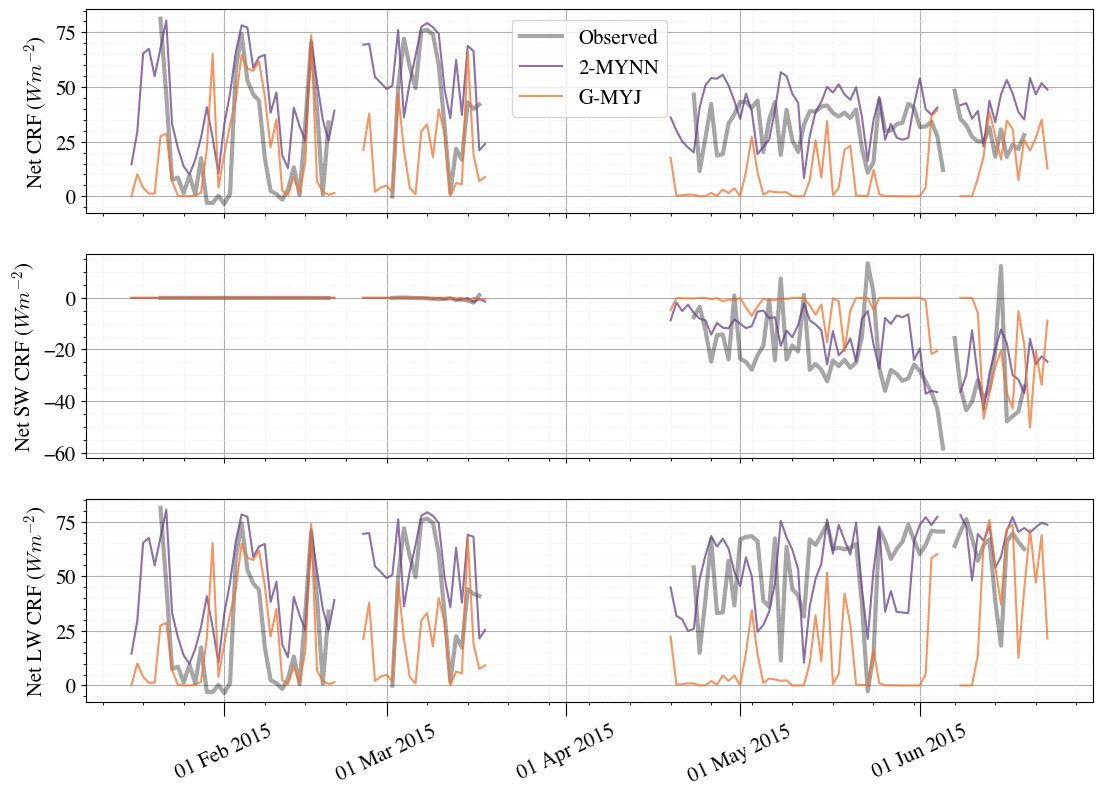
\includegraphics[width=1\linewidth]{figures/chapter4/CRF_TS.png}
    \caption[Time series of cloud radiative forcing in two WRF model runs.]{6-hourly net (top), longwave (bottom), and shortwave (middle) CRF from the N-ICE measurements (gray) and modeled by Polar WRF using the Morrison Two-Moment CM scheme with MYNN PBL scheme (purple) and the Goddard CM scheme with the MYJ PBL scheme (orange).}
    \label{fig:wrf_crf_all}
\end{figure}
\begin{figure}[p!]
    \centering
    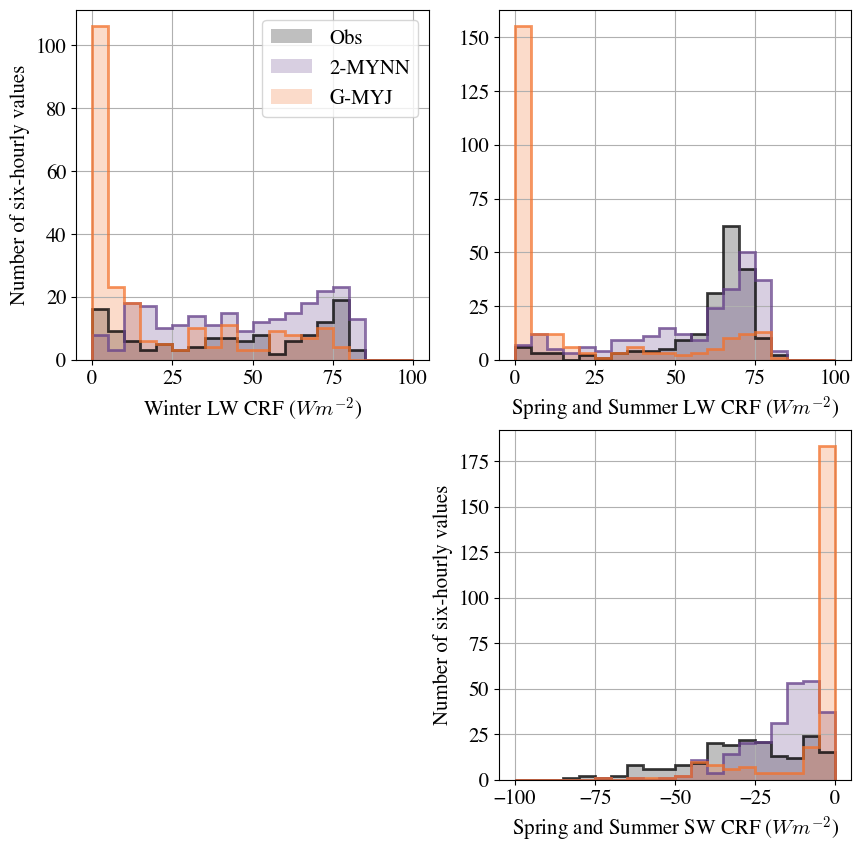
\includegraphics[width=1\linewidth]{figures/chapter4/CRF_Histos.png}
    \caption[Histograms of cloud radiative forcing in two WRF model runs.]{Longwave (top), and shortwave (bottom) CRF in the winter (left) and spring/summer (right). N-ICE measurements  are shown in black. Polar WRF simulated CRF from the Morrison Bulk Two-Moment CM scheme with MYNN PBL scheme (2-MYNN) and the Goddard CM scheme with the MYJ PBL scheme (G-MYJ) are shown in purple and orange.}
    \label{wrf:fig_crf_his}
\end{figure}

The 2-MYNN simulation slightly overestimates CRF throughout much of the N-ICE period. In the winter, CRF is estimated well during times when high CRF values were observed. The model does well with the low, thick clouds that produce high CRF values in the winter. However, in the spring and summer, this scheme underestimates the compensating shortwave CRF, resulting in net CRF values that are too high, regardless of how well the 2-MYNN scheme is reproducing the longwave forcing. The distribution of net longwave forcing can be seen in the top panels of Figure \ref{wrf:fig_crf_his} and the shortwave in the bottom panel.

The 2-MYNN scheme had the lowest longwave bias in the spring. However, the net shortwave bias was the largest with this scheme. Longwave CRF from 2-MYNN did capture some CRF peaks well in the spring, and much of the error in spring CRF is a result of the shortwave CRF. This indicates clouds at N-ICE had a greater influence on the shortwave radiation than those simulated by Polar WRF with the 2-MYNN configuration.

The G-MYJ simulation had the lowest sensible and latent heat flux biases in spring, but greatly underestimates all components of CRF. The G-MYJ simulation displays large net longwave biases. In the spring, the G-MYJ simulation significantly underestimated CRF until the last floe in June. Near the end of June, both model runs began to produce larger CRF values in both the longwave and shortwave. While this increase in longwave and shortwave CRF also increased the net CRF in the 2-MYNN scheme, it balances out to be around 25 $Wm^{-2}$ of net CRF in the G-MYJ scheme, which is similar to CRF values from the N-ICE measurements.

Even the schemes with the lowest biases in the turbulent fluxes simulate large inaccuracies in the modeled CRF. The modeled clouds are not producing the CRF required to replicate the measurements, indicating that the cloud properties are not simulated correctly. This could be caused by some combination of these properities: 1) too few clouds, 2) clouds are not warm enough, or 3) the clouds are not optically thick enough. It is most likely that the cloud fraction is too low because the shortwave flux during the transition from winter to spring is low, especially in the G-MYJ simulation. Figure \ref{fig:wrf_cloudfrac} in Chapter 3 supports this interpretation, showing cloud fraction in the G-MYJ simulation was consistently lower than the measurements, especially in the spring. This figure also shows that the 2-MYNN scheme underestimated cloud fraction throughout the entire spring period.

\section{Conclusions}
The N-ICE field campaign observed unique Arctic atmospheric conditions during the transition from winter to summer over first-year sea ice. As the Arctic continues to move toward ice-free conditions in summer, the need for observations over first-year sea ice becomes increasingly important. There is a need for sufficient measurements to provide valuable comparison datasets for models. Often, models' weaknesses lie in cloud properties. Particularly in the polar regions, where we have fewer observations for validation, the cloud properties are often unknown.

This study aimed to characterize the macrophysical and microphysical properties of the clouds at N-ICE. The cloud phase, base height, and base temperature were explored extensively both for the entire experiment, seasonally, and for a particularly uniquely strong storm-period. 

In the winter, the cloudy and clear conditions described in \citet{graham:2017:events} were clearly visible in the peaks in the distribution of longwave CRF around 0 $Wm^{-2}$ (clear) and again around 75 $Wm^{-2}$ (cloudy). Spring longwave CRF showed similar results, with an obvious clear and cloudy state. Shortwave CRF in the spring was negative for a lot of the season, with a few positive values in June. Spring and summer were characterized by low, primarily water clouds. Average cloud base height for each month in the spring and summer was below 3 $km$. Winter cloud base heights were higher, particularly those observed in January, when the average cloud base height was over 6 $km$ above the surface.

In winter, the cloud base height and temperature correlated with the CRF. Lower cloud base temperature generally indicated lower CRF values, as the clouds were higher, likely more optically thin, and colder. In the spring, the compensating effects of the LW and SW CRF can be seen. Lower cloud base heights produced increased longwave CRF (as warmer clouds increase LW radiation to the surface), but increased the magnitude of the (negative) shortwave CRF. The longwave influence dominated the CRF for the entire N-ICE experiment. 

Modeled CRF values from the polar WRF model were compared to CRF observations from N-ICE. Longwave CRF was underestimated by the model simulation using the G-MYJ configuration, with the most notable differences occurring during the spring. The 2-MYNN run also underestimated SW CRF, resulting in a significant underestimation of net CRF, regardless of this model performing well with latent and sensible heat flux calculations. The 2-MYNN run, the simulation with the lowest wintertime biases in chapter 3, produced LW CRF values similar to those observed at N-ICE. However, the SW CRF was underestimated by this simulation, resulting in a larger net CRF than was observed. In the winter, the 2-MYNN accurately predicts high CRF values but overpredicts low CRF values. In the spring, the opposite is true, higher CRF values are overestimated by the model, but lower CRF value clouds are relatively well modeled.

